% Options for packages loaded elsewhere
\PassOptionsToPackage{unicode}{hyperref}
\PassOptionsToPackage{hyphens}{url}
\PassOptionsToPackage{dvipsnames,svgnames,x11names}{xcolor}
%
\documentclass[
  letterpaper,
  DIV=11,
  numbers=noendperiod]{scrreprt}

\usepackage{amsmath,amssymb}
\usepackage{iftex}
\ifPDFTeX
  \usepackage[T1]{fontenc}
  \usepackage[utf8]{inputenc}
  \usepackage{textcomp} % provide euro and other symbols
\else % if luatex or xetex
  \usepackage{unicode-math}
  \defaultfontfeatures{Scale=MatchLowercase}
  \defaultfontfeatures[\rmfamily]{Ligatures=TeX,Scale=1}
\fi
\usepackage{lmodern}
\ifPDFTeX\else  
    % xetex/luatex font selection
\fi
% Use upquote if available, for straight quotes in verbatim environments
\IfFileExists{upquote.sty}{\usepackage{upquote}}{}
\IfFileExists{microtype.sty}{% use microtype if available
  \usepackage[]{microtype}
  \UseMicrotypeSet[protrusion]{basicmath} % disable protrusion for tt fonts
}{}
\makeatletter
\@ifundefined{KOMAClassName}{% if non-KOMA class
  \IfFileExists{parskip.sty}{%
    \usepackage{parskip}
  }{% else
    \setlength{\parindent}{0pt}
    \setlength{\parskip}{6pt plus 2pt minus 1pt}}
}{% if KOMA class
  \KOMAoptions{parskip=half}}
\makeatother
\usepackage{xcolor}
\setlength{\emergencystretch}{3em} % prevent overfull lines
\setcounter{secnumdepth}{5}
% Make \paragraph and \subparagraph free-standing
\ifx\paragraph\undefined\else
  \let\oldparagraph\paragraph
  \renewcommand{\paragraph}[1]{\oldparagraph{#1}\mbox{}}
\fi
\ifx\subparagraph\undefined\else
  \let\oldsubparagraph\subparagraph
  \renewcommand{\subparagraph}[1]{\oldsubparagraph{#1}\mbox{}}
\fi


\providecommand{\tightlist}{%
  \setlength{\itemsep}{0pt}\setlength{\parskip}{0pt}}\usepackage{longtable,booktabs,array}
\usepackage{calc} % for calculating minipage widths
% Correct order of tables after \paragraph or \subparagraph
\usepackage{etoolbox}
\makeatletter
\patchcmd\longtable{\par}{\if@noskipsec\mbox{}\fi\par}{}{}
\makeatother
% Allow footnotes in longtable head/foot
\IfFileExists{footnotehyper.sty}{\usepackage{footnotehyper}}{\usepackage{footnote}}
\makesavenoteenv{longtable}
\usepackage{graphicx}
\makeatletter
\def\maxwidth{\ifdim\Gin@nat@width>\linewidth\linewidth\else\Gin@nat@width\fi}
\def\maxheight{\ifdim\Gin@nat@height>\textheight\textheight\else\Gin@nat@height\fi}
\makeatother
% Scale images if necessary, so that they will not overflow the page
% margins by default, and it is still possible to overwrite the defaults
% using explicit options in \includegraphics[width, height, ...]{}
\setkeys{Gin}{width=\maxwidth,height=\maxheight,keepaspectratio}
% Set default figure placement to htbp
\makeatletter
\def\fps@figure{htbp}
\makeatother
\newlength{\cslhangindent}
\setlength{\cslhangindent}{1.5em}
\newlength{\csllabelwidth}
\setlength{\csllabelwidth}{3em}
\newlength{\cslentryspacingunit} % times entry-spacing
\setlength{\cslentryspacingunit}{\parskip}
\newenvironment{CSLReferences}[2] % #1 hanging-ident, #2 entry spacing
 {% don't indent paragraphs
  \setlength{\parindent}{0pt}
  % turn on hanging indent if param 1 is 1
  \ifodd #1
  \let\oldpar\par
  \def\par{\hangindent=\cslhangindent\oldpar}
  \fi
  % set entry spacing
  \setlength{\parskip}{#2\cslentryspacingunit}
 }%
 {}
\usepackage{calc}
\newcommand{\CSLBlock}[1]{#1\hfill\break}
\newcommand{\CSLLeftMargin}[1]{\parbox[t]{\csllabelwidth}{#1}}
\newcommand{\CSLRightInline}[1]{\parbox[t]{\linewidth - \csllabelwidth}{#1}\break}
\newcommand{\CSLIndent}[1]{\hspace{\cslhangindent}#1}

\KOMAoption{captions}{tableheading}
\makeatletter
\makeatother
\makeatletter
\@ifpackageloaded{bookmark}{}{\usepackage{bookmark}}
\makeatother
\makeatletter
\@ifpackageloaded{caption}{}{\usepackage{caption}}
\AtBeginDocument{%
\ifdefined\contentsname
  \renewcommand*\contentsname{Table of contents}
\else
  \newcommand\contentsname{Table of contents}
\fi
\ifdefined\listfigurename
  \renewcommand*\listfigurename{List of Figures}
\else
  \newcommand\listfigurename{List of Figures}
\fi
\ifdefined\listtablename
  \renewcommand*\listtablename{List of Tables}
\else
  \newcommand\listtablename{List of Tables}
\fi
\ifdefined\figurename
  \renewcommand*\figurename{Figure}
\else
  \newcommand\figurename{Figure}
\fi
\ifdefined\tablename
  \renewcommand*\tablename{Table}
\else
  \newcommand\tablename{Table}
\fi
}
\@ifpackageloaded{float}{}{\usepackage{float}}
\floatstyle{ruled}
\@ifundefined{c@chapter}{\newfloat{codelisting}{h}{lop}}{\newfloat{codelisting}{h}{lop}[chapter]}
\floatname{codelisting}{Listing}
\newcommand*\listoflistings{\listof{codelisting}{List of Listings}}
\makeatother
\makeatletter
\@ifpackageloaded{caption}{}{\usepackage{caption}}
\@ifpackageloaded{subcaption}{}{\usepackage{subcaption}}
\makeatother
\makeatletter
\@ifpackageloaded{tcolorbox}{}{\usepackage[skins,breakable]{tcolorbox}}
\makeatother
\makeatletter
\@ifundefined{shadecolor}{\definecolor{shadecolor}{rgb}{.97, .97, .97}}
\makeatother
\makeatletter
\makeatother
\makeatletter
\makeatother
\ifLuaTeX
  \usepackage{selnolig}  % disable illegal ligatures
\fi
\IfFileExists{bookmark.sty}{\usepackage{bookmark}}{\usepackage{hyperref}}
\IfFileExists{xurl.sty}{\usepackage{xurl}}{} % add URL line breaks if available
\urlstyle{same} % disable monospaced font for URLs
\hypersetup{
  pdftitle={FMA A-Team Manual},
  colorlinks=true,
  linkcolor={blue},
  filecolor={Maroon},
  citecolor={Blue},
  urlcolor={Blue},
  pdfcreator={LaTeX via pandoc}}

\title{FMA A-Team Manual}
\author{}
\date{2023-07-19}

\begin{document}
\maketitle
\ifdefined\Shaded\renewenvironment{Shaded}{\begin{tcolorbox}[frame hidden, boxrule=0pt, sharp corners, interior hidden, breakable, borderline west={3pt}{0pt}{shadecolor}, enhanced]}{\end{tcolorbox}}\fi

\renewcommand*\contentsname{Table of contents}
{
\hypersetup{linkcolor=}
\setcounter{tocdepth}{2}
\tableofcontents
}
\bookmarksetup{startatroot}

\hypertarget{fma-a-team-manual}{%
\chapter{FMA A-Team Manual}\label{fma-a-team-manual}}

Welcome!\footnote{This website is a collaborative effort of the FMA
  A-Team, with input from AFSC FMA Division staff.}

This is the manual for the Analytical Services Program in the Fisheries
Monitoring and Analysis Division at NOAA's Alaska Fisheries Science
Center\footnote{Jeepers, that's a mouthful! Let's just abbreviate from
  now on - acronym definitions are
  \protect\hyperlink{sec-acronyms}{here}}.

The focus of our work centers on providing scientific products to
support the management of marine ecosystems and commercial fisheries.

This manual is intended to provide an overview for Program staff and
others about how we do our work, and our expectations It is also a space
to document institutional knowledge and for important information about
procedures and available resources. If you have suggestions for
additions or changes, please contact the Analytical Services Program
Manager, Jason Jannnot (jason.jannot@noaa.gov), make a pull request, or
submit an issue.

\bookmarksetup{startatroot}

\hypertarget{intro}{%
\chapter{Introduction}\label{intro}}

The FMA Analytical Services Team adheres to NOAA's mission of
\href{https://www.noaa.gov/our-mission-and-vision}{Science, Service, and
Stewardship}.

In short, our mission is\ldots{}\textbf{INSERT SUMMARY OF MISSION FROM
\protect\hyperlink{sec-big-picture}{HERE}}

See \protect\hyperlink{sec-big_picture}{The Big Picture} section for
more detail on our culture and philosophy.

We are motivatedby\ldots{} \textbf{INSERT MOTIVATIONAL
REFERENCES}\ldots:

\hypertarget{how-we-meet}{%
\section{How we meet}\label{how-we-meet}}

\hypertarget{a-team-meetings}{%
\subsection{A-Team Meetings}\label{a-team-meetings}}

\hypertarget{semimonthly-thursdays-1000-pt-google-meet}{%
\subsubsection{semimonthly Thursdays, 1000 PT, Google
Meet}\label{semimonthly-thursdays-1000-pt-google-meet}}

Currently, as a whole team, we meet virtually by Google Meet every 2
weeks. We use Google Docs to set agendas, record decisions made, and
outline action items during these meetings.

\hypertarget{with-jason}{%
\subsection{1:1 with Jason}\label{with-jason}}

We each have individual in-person meetings with Jason.\\
Each member is responsible for documenting their 1:1 meetings with
Jason, including tracking decisions and action items for themselves.
Jason is happy to collaborate in Google Docs with individuals if that is
their desire.

\hypertarget{how-we-give-feedback}{%
\section{How we give feedback}\label{how-we-give-feedback}}

Feedback, both giving and receiving it, is an important aspect of our
team. We expect feedback to be supportive but constructive. Feedback we
give and receive can come in a variety of places and times, including
but not limited to, during: brainstorming sessions; meetings; reviews of
code or written documents; practice talks; post-project/post-meeting
debriefs; 1:1's with Jason.

This
\href{https://scwrl.ubc.ca/stem-writing-resources/learning-strategies-for-communicating-science/how-to-give-and-receive-effective-feedback/}{resource
from UBC} outlines best practices for giving and receiving feedback.

\hypertarget{how-we-share-things}{%
\section{How we share things}\label{how-we-share-things}}

We think it is useful to have standard ways of sharing things. These
don't always have to be followed but are a useful guide. The most
important principle is to make it easier for others and your future
self!

\begin{itemize}
\tightlist
\item
  Mechanisms for Sharing

  \begin{itemize}
  \tightlist
  \item
    Code: Github (preferred), Google Docs

    \begin{itemize}
    \tightlist
    \item
      GitHub account:
      \href{https://github.com/Alaska-Fisheries-Monitoring-Analytics}{Alaska
      Fisheries Monitoring Analytics}\\
    \end{itemize}
  \item
    Docs: Rmarkdown (preferred), Google Docs, or MSWord

    \begin{itemize}
    \tightlist
    \item
      \href{https://github.com/Alaska-Fisheries-Monitoring-Analytics/ateam-manual}{A-team
      Manual}\\
    \end{itemize}
  \item
    Network Drives

    \begin{itemize}
    \tightlist
    \item
      \texttt{Y://Programs\ Share/FMA\_Observers/Observer/A\ is\ for\ ANALYSIS/}\strut \\
    \item
      Google Drive: \texttt{FMA\ Analysis\ Group} (request access)
    \end{itemize}
  \item
    FMAnalytics G-Chat Space\\
  \item
    project specific G-Chat Spaces (e.g., SASH, ADP)\\
  \item
    Github Issues\\
  \end{itemize}
\item
  When sharing make sure to describe what you are sharing\\
\item
  A project-based approach to organizing your work makes it easier to
  share and solicit feedback from others

  \begin{itemize}
  \tightlist
  \item
    here is
    \href{https://www.r-bloggers.com/2018/08/structuring-r-projects/}{is
    a good guide}\\
  \item
    see also \emph{Good enough practices in scientific computing}
    (Wilson et al. 2017))
  \end{itemize}
\end{itemize}

See the \protect\hyperlink{resources}{Resources} section for other
useful resources

\hypertarget{references}{%
\section{References}\label{references}}

\bookmarksetup{startatroot}

\hypertarget{sec-big-picture}{%
\chapter{The Big Picture}\label{sec-big-picture}}

\hypertarget{vision---where-are-we-going}{%
\section{Vision - Where are we
going?}\label{vision---where-are-we-going}}

\begin{quote}
Team Core Values - Taken from the ADP Charter Collaboration -
conversation, not lecturing Flexibility - kill your darlings for the
greater good if necessary. Respect - we are all professionals and should
be treated as such. Safety - the group space is safe for productive
conflict Humor - don't take anything too seriously Kindness - don't be a
jerk
\end{quote}

\begin{itemize}
\tightlist
\item
  What is the future state of the team? What does it look like?
\item
  Answers the question: Where are you going?
\item
  If there were no constraints at all, what would things look like in 5
  years, 10 years, 20 years?
\item
  What picture do we want to create for the future?
\item
  What legacy do we want to leave behind? Aim for a vivid picture of
  what the future looks like in 2-3 pages
\end{itemize}

What does success look like for the team?

\hypertarget{purpose---why-do-we-do-this}{%
\section{Purpose - Why do we do
this?}\label{purpose---why-do-we-do-this}}

Why does the team exist? What is the inspiration that guides and
motivates the team to achieve the mission?

\hypertarget{mission---what-do-we-do}{%
\section{Mission - What do we do?}\label{mission---what-do-we-do}}

What the team aims to do to fulfill its purpose and acheive it's vision.

\hypertarget{internal-stakeholders}{%
\section{Internal Stakeholders}\label{internal-stakeholders}}

\hypertarget{external-stakeholders}{%
\section{External Stakeholders}\label{external-stakeholders}}

\hypertarget{culture-values}{%
\section{Culture \& Values}\label{culture-values}}

\begin{itemize}
\tightlist
\item
  Share our learning and time with others on the team as well as those
  beyond our team, knowing that this builds community and ultimately
  improves both the quality and impact of our science.
\end{itemize}

\bookmarksetup{startatroot}

\hypertarget{code}{%
\chapter{Code of Conduct}\label{code}}

A \emph{Code of Conduct} is a set of basic ground rules that we ask team
members to follow. The goal is to create an open and inclusive space for
our work that helps us achieve our collective goals. Along with our
\protect\hyperlink{sec-big_picture}{Big Picture}, a \emph{Code of
Conduct}

\begin{itemize}
\tightlist
\item
  provides a benchmark for self-evaluation\\
\item
  helps define our identity\\
\item
  establishes behavioral guidelines
\end{itemize}

\textbf{We expect all team members to adhere to the policies and
guidelines outlined here, as well as those found in the
\href{https://drive.google.com/file/d/1wV0g2Tea0jdPjsTeNNST7I871j70qLAw/view}{AFSC
Code of Conduct}.}

\textbf{\emph{The FMA Analytical Services Team is dedicated to providing
a harassment-free experience for everyone, regardless of gender, gender
identity and expression, sexual orientation, disability, physical
appearance, body size, age, race, or religion. We do not tolerate
harassment of team members or others in our larger communities in any
form.}}

This code of conduct applies to all A-Team spaces, including group and
individual meetings (face to face and remote), workshops, email
correspondence, chat and web channels, and code repositories. Anyone who
violates this code of conduct may be sanctioned and referred to the
AFSC's policies.

\hypertarget{reporting}{%
\subsection{Reporting}\label{reporting}}

If you are being harassed by a member of the FMA A-Team, notice that
someone else is being harassed, or have any other concerns, please
contact the FMA Analytical Services Program Manager, Dr.~Jason Jannot,
at
\href{mailto:jason.jannot@noaa.gov}{\nolinkurl{jason.jannot@noaa.gov}}.
If you do not feel comfortable reporting to Jason, please contact
Jennifer Ferdinand (FMA Division Director) or Lisa Thompson (FMA Deputy
Director) or any other AFSC supervisor. Other methods of reporting
available to you include:

\begin{itemize}
\tightlist
\item
  \href{https://noaasashhelpline.org/}{NOAA Sexual Assault Sexual
  Harassment Helpline}
\item
  \href{https://www.noaa.gov/workplace-violence-prevention-response-program}{NOAA
  Workplace Violence Prevention and Response Program}
\item
  \href{mailto:DAO-955.OHCS@noaa.gov}{NOAA Workforce Management Office}
\item
  \href{mailto:noaa.oicr@noaa.gov}{NOAA Office of Inclusion and Civil
  Rights}
\end{itemize}

In addition to the AFSC's Code of Conduct, the Dec.~8th 2022
\href{https://www.noaa.gov/organization/inclusion-and-civil-rights/policy-statement-on-equal-employment-opportunity}{Policy
Statement on Equal Employment Opportunity} from NOAA provides a good
explanation of NOAA's stance and policies against harassment,
discrimination, and violence in the workplace.

\bookmarksetup{startatroot}

\hypertarget{onboarding}{%
\chapter{Onboarding}\label{onboarding}}

Welcome to the FMA A-Team!

\includegraphics{200.webp}

Here are some resources to help you get settled.

Our group is excited that you have decided to join our team! We hope
that these onboarding resources, guidelines, and tips will make your
transition to FMA seamless and enjoyable.

\href{https://drive.google.com/file/d/1Gxg-tw76NeptYFkya7M6JSyxsy31mmAu/view?usp=sharing}{AFSC
Onboarding Checklist for Federal and Non-Federal Staff}

The
\href{https://drive.google.com/drive/folders/1aZcoJooHxNMh4kjCiv4WUgpDtszub1PI}{New
Employee Onboarding} Google Drive folder has many good resources.

\hypertarget{cac}{%
\section{CAC}\label{cac}}

A CAC will give you access to buildings and computer systems. It is the
necessary first step to getting started.

\hypertarget{get-a-new-cac}{%
\subsection{Get a New CAC}\label{get-a-new-cac}}

CAC cards are only issued at Defense Department authorized locations
(referred to as ``RAPIDS'' offices) and may or may not be associated
with a NOAA facility. For AFSC staff, the following locations are the
closet RAPIDS stations.

\begin{enumerate}
\def\labelenumi{\arabic{enumi}.}
\item
  Seattle staff = WRC building 1, site ID 105831 (phone: 206-526-6571)
\item
  Juneau staff = Federal Bldg, site 102444 (phone: 907-463-2170)
\end{enumerate}

\hypertarget{renew-a-cac}{%
\subsection{Renew a CAC}\label{renew-a-cac}}

See the
\href{https://sites.google.com/noaa.gov/myafsc/administrative/security/cac-renewal}{CAC
Renewal page} on MyAFSC

\hypertarget{it}{%
\section{IT}\label{it}}

On the first day, an A-Team member (likely Jason), will bring you to
OFIS to:

\begin{itemize}
\tightlist
\item
  get computer equipment
\item
  set-up accounts (including an Oracle database account)
\item
  get logged into NOAA computer \& Google account
\item
  request VPN accounts
\item
  download software needed (e.g., R, RStudio, SQL Developer, Endnote)
\item
  check the
  \href{https://sites.google.com/noaa.gov/myafsc/technology/onboarding-and-clearing-it}{IT
  Onboarding webpage} for more information
\end{itemize}

\href{https://sites.google.com/noaa.gov/myafsc/technology}{IT Resources}
\href{https://sites.google.com/noaa.gov/myafsc/technology/afsc-it-service-desk}{IT
Help}

\hypertarget{schedules-time-attendance}{%
\section{Schedules, Time \&
Attendance}\label{schedules-time-attendance}}

You will access your timesheets through the
\href{https://docwebta.eas.commerce.gov/webta/}{GovTA} web portal.
Within one week of on-boarding
\href{https://enterpriseservices.servicenowservices.com/es}{Enterprise
Services} will create a new profile for you in webTA/GovTA.

You should:

\begin{itemize}
\tightlist
\item
  work with Jason to set your work schedule\\
\item
  familiarize yourself with the defintions and rules around
  \href{https://drive.google.com/file/d/1VlxkCEHZEdQd2pfGu9Bud5QZDUudqioa/view?pli=1}{Alternative
  Work Schedules}\\
\item
  fill out an
  \href{https://drive.google.com/file/d/1SvyTE2M6lQ0dcX5w3b0f7CJNxU6zDFDy/view?usp=share_link}{Employee
  Work Schedule Form}\\
\item
  fill out a
  \href{https://drive.google.com/file/d/19oABvmjMgRX4az-9U1Ijgd3ux5BwmHQw/view}{Telework
  Application Agreement}\\
\item
  fill out a Telework Application Routing form
\item
  take the CLC Telework Training
\end{itemize}

Forms and information can be found on the
\href{https://sites.google.com/noaa.gov/myafsc/administrative/time-and-attendance}{myAFSC
Time and Attendance page}

\href{https://sites.google.com/noaa.gov/myafsc/administrative/time-and-attendance}{Time
and Attendance Resouces}

\hypertarget{leave}{%
\subsection{Leave}\label{leave}}

Use GovTA to request leave. You can find resources related to leave
\href{https://sites.google.com/noaa.gov/myafsc/administrative/time-and-attendance}{here}

\hypertarget{compensatory-time}{%
\subsection{Compensatory Time}\label{compensatory-time}}

In most cases, compensatory time can be awarded for travel that occurs
outside or beyond normal working hours or days.

Compensatory time for working (as opposed to traveling) is typically not
awarded. Rather, overtime work is typically compensated via overtime
pay.

A quick guide for how to claim and record Compensatory Time can be found
\href{https://docs.google.com/document/d/1BdvL0mbBE0JY5HkDjdoi5RhCc0rn3G0SfXFHeo03nzY/edit}{here}.

\hypertarget{sec-perf}{%
\section{Performance}\label{sec-perf}}

Soon after joining the A-Team, you should work with the PM to create an
annual, individual
\href{https://drive.google.com/file/d/18veCUTjncQVhRY6jOou9kclKWXJssOca/view?pli=1}{Performance
Plan}. Specific responsibilities, individual projects, deliverables, and
duties will be reflected in the individual Performance Plan. This
document will guide your work and will be revisited (in discussions with
the PM) during the year and updated to reflect any changes on an annual
basis.

Duties that team members might assume, depending on interest, time,
Program/Division/Center priorities, and needs include (but are not
limited to):

\begin{itemize}
\tightlist
\item
  leading and assisting in designated research projects\\
\item
  participation in professional development opportunities\\
\item
  developing and submitting research funding proposals\\
\item
  submitting and publishing NOAA Technical Memorandum and other
  reports\\
\item
  submitting and publishing peer-reviewed journal articles
\item
  participating in outreach activities\\
\item
  attending scientific and professional conferences
\end{itemize}

More about the performance process can be found
\href{https://sites.google.com/noaa.gov/inside-fisheries-hc/human-capital/performance-culture-incentive-and-honorary-awards/commerce-alternative-personnel-system-caps}{here}.

The
\href{https://sites.google.com/noaa.gov/myafsc/administrative/workforce-management/awards}{AFSC
Awards page} lists the many ways you can be recognized and awarded for
your achievements as well as opportunities to nominate your peers for
their hard work.

\hypertarget{facilities}{%
\section{Facilities}\label{facilities}}

AFSC buildings on the Seattle Sand Point Campus (a.k.a.
\href{https://www.wrc.noaa.gov/}{Western Regional Center {[}WRC{]}}) are
only accessible during work hours and with a CAC.

\hypertarget{office-space}{%
\subsection{Office space}\label{office-space}}

Our physical offices are in Building 4 of the WRC.\\
The following are FMA A-Team (and affiliated staff) office numbers:

\begin{itemize}
\tightlist
\item
  1060 -
  \href{https://www.fisheries.noaa.gov/contact/jason-e-jannot}{Jason
  Jannot, FMA Analytical Services Program Manager}
\item
  1057 - Lacey Jeroue, AMMOP Program Manager
\item
  1057 - Andy Kingham, Analyst/IT developer
\item
  1057 - Geoff Mayhew, Research Fishery Biologist
\item
  1056 -
  \href{https://www.fisheries.noaa.gov/contact/craig-h-faunce}{Craig
  Faunce, Research Fisheries Biologist}
\item
  1089 - Jennifer Cahalan, Statistician/Analyst
\item
  \href{https://www.fisheries.noaa.gov/contact/phil-ganz}{Phil Ganz},
  \href{https://www.fisheries.noaa.gov/contact/jason-gasper-phd}{Jason
  Gasper},
  \href{https://www.fisheries.noaa.gov/contact/jennifer-mondragon}{Jennifer
  Mondragon} all work in the AKRO in Juneau and work closely with the
  FMA A-Team.
\end{itemize}

Other FMA staff offices

\begin{itemize}
\tightlist
\item
  1059 -
  \href{https://www.fisheries.noaa.gov/contact/jennifer-ferdinand}{Jennifer
  Ferdinand, FMA Division Director}
\item
  1061 -
  \href{https://www.fisheries.noaa.gov/contact/lisa-thompson}{Lisa
  Thompson, FMA Deputy Director}
\item
  1062 -
  \href{https://www.fisheries.noaa.gov/contact/marlon-concepcion}{Marlon
  Conception, FMA Debriefing Program Manager}
\item
  1063 - \href{https://www.fisheries.noaa.gov/contact/brian-mason}{Brian
  Mason, FMA Training Program Manager}
\end{itemize}

\hypertarget{reservations}{%
\subsection{Reservations}\label{reservations}}

Reservations for rooms or government vehicles can be found
\href{https://sites.google.com/noaa.gov/myafsc/reservations}{here}

\hypertarget{parking}{%
\subsection{Parking}\label{parking}}

To obtain either a vehicle or a bike parking pass for the Seattle Sand
Point Campus, contact Pass \& ID Security Office in Building 1
(206-526-6571). You will need to fill out a
\href{http://www.google.com/url?q=http\%3A\%2F\%2Fwww.wrc.noaa.gov\%2Fforms\%2FWRC\%2520Parking\%2520Decal\%2520v2008a.pdf\&sa=D\&sntz=1\&usg=AOvVaw2YdnFqmKoV029T-pt6UwFj}{WRC
Parking Form}.

\hypertarget{transit-benefits-for-bicyclists}{%
\subsection{Transit Benefits for
Bicyclists}\label{transit-benefits-for-bicyclists}}

Allows for reimbursement to employees who use a non-motorized bicycle
for a substantial portion of travel between your residence and the
worksite. Reimbursement can be up to \$20 per month, not to exceed \$240
per calendar year for bicycle commuting expenses.

\href{https://sites.google.com/noaa.gov/cao/about-ocao/logistics-operations-division/noaa-transit-subsidy-program}{More
information on bike benefits and instructions}.

\hypertarget{transportation-subsidy}{%
\subsection{Transportation Subsidy}\label{transportation-subsidy}}

NOAA offers this non-taxable transit-fare subsidy program to encourage
federal employees to use public mass transportation while commuting to
and from work. Qualified employees are provided with a monthly benefit
based on the distance to and from work. The monthly maximum subsidy
transit benefit allowance is \$270. Unused benefits do not carry over to
the next month.

\href{https://sites.google.com/noaa.gov/cao/about-ocao/logistics-operations-division/noaa-transit-subsidy-program}{More
information on the transit subsidy program and application.}

\hypertarget{afsc-contact-card}{%
\section{AFSC Contact Card}\label{afsc-contact-card}}

You are encouraged to set-up an AFSC Contact Card, for example, see
\href{https://www.fisheries.noaa.gov/contact/jason-e-jannot}{Jason's
Contact Card}. This is optional and not required but provides a public
facing profile so that others within and outside NOAA can find you and
can be linked to other social media accounts (e.g., Research Gate,
LinkedIn, etc.). You can request a
\href{https://docs.google.com/forms/d/e/1FAIpQLSdDfxoDycZjcmXDfPY_KnHwb2vPQ8HTzfFCSVt-qOvq_xPIZw/viewform}{Contact
Card here}

\hypertarget{general-adminstrative-resources}{%
\section{General Adminstrative
Resources}\label{general-adminstrative-resources}}

\href{https://sites.google.com/noaa.gov/myafsc/administrative/general-admin}{General
Admin Resources}

\hypertarget{health-safety}{%
\section{Health \& Safety}\label{health-safety}}

\href{https://sites.google.com/noaa.gov/myafsc/covid-19}{COVID
reporting}

Other health and safety resources (e.g., reporting an accident) can be
found \href{https://sites.google.com/noaa.gov/myafsc/safety}{here}.

\bookmarksetup{startatroot}

\hypertarget{expectations}{%
\chapter{Expectations}\label{expectations}}

\hypertarget{availability}{%
\section{Availability}\label{availability}}

\begin{itemize}
\tightlist
\item
  Core hours for the AFSC are 9:30 am to 2:30 pm, T,W,R.\\
\item
  A-Team members are encouraged to work in the office on one or more of
  these days.\\
\item
  Core hours do not apply on Monday or Friday.
\end{itemize}

You are \textbf{not} expected to be available 24/7. Similarly, unless it
is an emergency, do not expect responses to emails or any communication
before or after regular business hours on weekdays (6 am - 6 pm), or any
time on weekends/holidays/flex-days. However, because we recognize that
A-Team members should be able to create a working schedule that is right
for them, team members will not be penalized for sending communication
outside normal working hours.

\hypertarget{google}{%
\section{Google}\label{google}}

\hypertarget{g-mail}{%
\subsection{G-Mail}\label{g-mail}}

We communicate largely via email on the A-Team. You should therefore
check your email at least once a day during the normal work week.

\hypertarget{g-calendar}{%
\subsection{G-Calendar}\label{g-calendar}}

Much of our work is communicating and much of that communication comes
in the form of meetings. Therefore, you should:

\begin{itemize}
\tightlist
\item
  \protect\hyperlink{sec-calendar}{Make your calendar visible} to
  others.\\
\item
  Keep your calendar up-to-date\\
\item
  Add your working location and hours\\
\item
  Add leave and out of office (OOO)\\
\item
  Set-up automated OOO messages with alternative contacts, if OOO for
  longer than 1 day
\end{itemize}

\hypertarget{attendance-at-regularly-scheduled-events}{%
\section{Attendance at regularly scheduled
events}\label{attendance-at-regularly-scheduled-events}}

Attendance, either virtual or in-person, is reasonably expected at:

\begin{itemize}
\tightlist
\item
  Semimonthly A-Team meetings
\item
  Individual 1:1 with Jason (in-person when possible)
\item
  Regularly scheduled project meetings\\
\item
  NPFM Council Meetings\\
\item
  FMA All-hands
\end{itemize}

Attendance is strongly recommended when possible at:

\begin{itemize}
\tightlist
\item
  AFSC All-Hands\\
\item
  Other Center-wide Meetings
\end{itemize}

\hypertarget{expectations-of-the-program-manager}{%
\section{Expectations of the Program
Manager}\label{expectations-of-the-program-manager}}

As of \texttt{r\ format(Sys.Date(),\ "\%Y")}, Jason Jannot is the FMA
Analytical Program Manager. You can read about his
\protect\hyperlink{sec-jj-philosophy}{leadership and management
philosophy here}.

The Program Manager will (at a minimum) provide the A-Team with:

\begin{itemize}
\tightlist
\item
  Clarity (the \texttt{why?})
\item
  Guidance (the \texttt{how?})\\
\item
  Expectations (the \texttt{what?})\\
\item
  Collaboration \& Communication (the \texttt{who?})
\item
  Prioritization \& Gate-keeping\\
\item
  Accountability\\
\item
  Visibility \& Public Recognition\\
\item
  Overcoming Barriers\\
\item
  Timely Administrative Support
\end{itemize}

In addition to the above, the Program Manager will (at a minimum)
provide individual team members with:

\begin{itemize}
\tightlist
\item
  Positive feedback \& constructive criticism on work\\
\item
  Professional career support and development, including but not limited
  to:

  \begin{itemize}
  \tightlist
  \item
    opportunities for

    \begin{itemize}
    \tightlist
    \item
      training\\
    \item
      presenting (e.g., conferences, meetings, outreach, etc.)\\
    \item
      publishing
    \item
      advancing (e.g., promotion, details, etc.)\\
    \item
      collaborating\\
    \item
      leading\\
    \item
      mentoring
    \end{itemize}
  \end{itemize}
\item
  Regular meetings to discuss work \& maintain progress on goals\\
\item
  Empathetic listening\\
\item
  Coaching
\end{itemize}

\hypertarget{expectations-of-team-members}{%
\section{Expectations of Team
Members}\label{expectations-of-team-members}}

A-Team members will (at minimum):

\begin{itemize}
\tightlist
\item
  strive to produce the best science, given the constraints\\
\item
  grow and maintain technical and inter-personal skills
\item
  share knowledge, experience, code, and time
\item
  adopt a collaborative working mindset\\
\item
  adapt and be flexible, within reason\\
\item
  communicate clearly and effectively
\item
  communicate both successes and sticking points regularly\\
\item
  contribute to creating a positive, inclusive, and safe work culture
\end{itemize}

Remember, as a government agency, we serve the people of the United
States and service is 1/3\textsuperscript{rd} of
\href{https://www.noaa.gov/our-mission-and-vision}{NOAA's mission}.
Adopting a service mindset when approaching each other, stakeholders,
partners, and collaborators will magnify our positive impacts on marine
ecosystems, commercial fishing, and the wider world.

Some ways to adopt a service mindset:

\begin{itemize}
\tightlist
\item
  Mentor others when appropriate, especially new team members\\
\item
  Serve as a role model\\
\item
  Serve as a resource for other members of the A-Team\\
\item
  Nominate your peers for their hard work and achievements -
  \href{https://sites.google.com/noaa.gov/myafsc/administrative/workforce-management/awards}{AFSC
  Awards page}.
\item
  Participate in outreach activities
\end{itemize}

\hypertarget{team-collaboration-and-communication}{%
\section{Team Collaboration and
Communication}\label{team-collaboration-and-communication}}

Although the Program Manager is your primary supervisor, everyone should
always feel like they can reach out to anyone else on the A-team for
help or collaboration.

\bookmarksetup{startatroot}

\hypertarget{communication}{%
\chapter{Communication}\label{communication}}

There is a plethora of communication methods and technologies. However,
the communication tool should be chosen based on the purpose of the
communication. The purpose of this document is to explain how
communication tools differ so that the tool used is appropriate given
the topic(s) and timelines.

\hypertarget{email}{%
\section{Email}\label{email}}

\textbf{Topics}: Single topics requiring little/no context, explanation,
or discussion\\
\textbf{Time}:

\begin{itemize}
\tightlist
\item
  Immediate action is not required and/or;\\
\item
  Discussion is very limited or unnecessary and/or;\\
\item
  Completion time is not pressing
\end{itemize}

\textbf{Tone}: It can be very difficult to get the right tone in an
email. Sometimes it's worthwhile to write the email but delay sending
it. Then go back and check the tone after taking a pause.\\
\textbf{Pros}: Creates a record\\
\textbf{Cons}: Can be slow, lost, ignored\\
\textbf{Tracking}: Formally captured in writing - creates a record\\
\textbf{Uses}:

\begin{itemize}
\tightlist
\item
  Simple requests for a single action or, at most, a few closely related
  actions\\
\item
  Short summary of a single topic\\
\item
  Routine tasking\\
\item
  Follow-up summaries from video calls/FTF/phone calls
\end{itemize}

\textbf{Consider}: moving to a video call/FTF or phone call if the email
chain goes back and forth more than a few times or in-depth discussion
is necessary.

\hypertarget{video-callface-to-face-meeting-ftf}{%
\section{Video call/Face-To-Face Meeting
(FTF)}\label{video-callface-to-face-meeting-ftf}}

\textbf{Topics}: Sensitive, complex, or multiple topics\\
\textbf{Time}: Lengthy discussion necessary; actions or responses will
be discussed\\
\textbf{Tone}: Voice inflection, body language and body posture can be
distorted or hidden by the tech. Eye contact can be misinterpreted,
misleading, or absent.\\
\textbf{Pros}: Can screen share/show\\
\textbf{Cons}: Requires some planning\\
\textbf{Tracking}: No formal tracking - requires participants to take
notes; Video calls can be recorded.\\
\textbf{Use}:

\begin{itemize}
\tightlist
\item
  To collaborate with team members\\
\item
  To build rapport and relationships\\
\item
  To provide or receive feedback\\
\item
  To provide or receive coaching\\
\item
  For instructional/side-by-side training/teaching\\
\item
  When there are multiple participants\\
\item
  When screen sharing/showing is needed
\end{itemize}

\textbf{Consider}: using other methods for simple updates that are
informational only and require no response.

\hypertarget{chat}{%
\section{Chat}\label{chat}}

\textbf{Topics}: Single, non-sensitive topics\\
\textbf{Time}:

\begin{itemize}
\tightlist
\item
  Immediate response is necessary, requested or implied
\item
  Discussion is very limited or unnecessary
\item
  Very simple responses expected
\end{itemize}

\textbf{Tone}: Fast pace can lead to misunderstandings of tone and
intent, similar to email.\\
\textbf{Pros}: Fast\\
\textbf{Cons}:

\begin{itemize}
\tightlist
\item
  No record created\\
\item
  Limited ability to engage in depth\\
\item
  Links to files will be lost if history is turned off
\end{itemize}

\textbf{Tracking}: No formal tracking - requires participants to take
notes or screen shots.\\
\textbf{Use}:

\begin{itemize}
\tightlist
\item
  To ask simple questions\\
\item
  To check-in for current/near-future availability\\
\item
  Share informational link\\
\item
  Real-time discussion among team during formal meetings, e.g., FMAC,
  PCFMAC, Council, etc. - though discussion will be limited
\end{itemize}

\textbf{Consider}: moving lengthy discussions to a video call or FTF.

\hypertarget{phone}{%
\section{Phone}\label{phone}}

\textbf{Topics}: Sensitive or complex topics\\
\textbf{Time}:

\begin{itemize}
\tightlist
\item
  Immediate response or action is necessary\\
\item
  Discussion could be lengthy\\
\item
  Completion time is pressing
\end{itemize}

\textbf{Tone}: Voice inflection can be distorted, lost or misinterpreted
due to tech; requires careful listening and voice control.\\
\textbf{Pros}: Can address time sensitive issues quickly\\
\textbf{Cons}: No screen show/share, body language missing\\
\textbf{Tracking}: No formal tracking - requires participants to take
notes\\
\textbf{Use}:

\begin{itemize}
\tightlist
\item
  Emergencies\\
\item
  Urgent, time sensitive requests\\
\item
  Contact necessary during off-hours or off-days\\
\item
  When video call/FTF is not possible but topics are sensitive or
  complex\\
\item
  Quick topics that are time sensitive
\end{itemize}

\textbf{Consider}: following up with an email summary of the
conversation

\hypertarget{mobile-textsms}{%
\section{Mobile Text/SMS}\label{mobile-textsms}}

\textbf{Topics}: Extremely time sensitive\\
\textbf{Time}:

\begin{itemize}
\tightlist
\item
  Immediate response or action is necessary
\item
  No discussion
\item
  Very simple responses expected
\end{itemize}

\textbf{Tone}: Fast pace can lead to misunderstandings of tone and
intent, similar to email and chat.\\
\textbf{Pros}: Can address time sensitive issues quickly\\
\textbf{Cons}: No screen show/share\\
\textbf{Tracking}: Creates a record, but there might be limits and
constraints\\
\textbf{Use}:

\begin{itemize}
\tightlist
\item
  Emergencies\\
\item
  Urgent, time sensitive requests\\
\item
  Necessary contact during off-hours or off-days\\
\item
  To check-in for current/near-future availability
\end{itemize}

\textbf{Consider}: moving to another method as soon as practicable.

\bookmarksetup{startatroot}

\hypertarget{sec-projects}{%
\chapter{Projects}\label{sec-projects}}

\hypertarget{intake}{%
\section{Intake}\label{intake}}

\href{https://docs.google.com/spreadsheets/d/1MXWbgYy-91S_PvldipatwdodjIjBECVL5yuWkLVIw50/edit?usp=sharing}{Project
Intake} (google sheet 1)

\href{https://docs.google.com/spreadsheets/d/1MXWbgYy-91S_PvldipatwdodjIjBECVL5yuWkLVIw50/edit?usp=sharing}{FY24
NOAA Priorities} (google sheet 3)

\hypertarget{prioritization}{%
\section{Prioritization}\label{prioritization}}

\href{https://docs.google.com/spreadsheets/d/1MXWbgYy-91S_PvldipatwdodjIjBECVL5yuWkLVIw50/edit?usp=sharing}{Project
Prioritization} (google sheet 2)

\hypertarget{planning}{%
\section{Planning}\label{planning}}

\hypertarget{tools-workflow}{%
\section{Tools \& Workflow}\label{tools-workflow}}

\href{081-code-review.qmd}{Code Review}

\hypertarget{completion}{%
\section{Completion}\label{completion}}

\hypertarget{debrieflessons-learned}{%
\section{Debrief/Lessons Learned}\label{debrieflessons-learned}}

\bookmarksetup{startatroot}

\hypertarget{offboarding}{%
\chapter{Offboarding}\label{offboarding}}

\href{https://drive.google.com/file/d/17hBFFWaAImoVNqHfPJmoAKqGqs8rD1Q2/view?usp=sharing}{AFSC
Offboarding Checklist for Federal Staff}

\href{https://drive.google.com/file/d/1BdNN2rvgwdyUAuk_9cOlRGw5_ik6K37Q/view?usp=sharing}{AFSC
Offboarding Checklist for Non-Federal Staff (contractors and
affiliates)}

\hypertarget{exit-interview}{%
\section{Exit Interview}\label{exit-interview}}

Set up a dedicated time to meet with the A-Team PM to talk about your
time in FMA, and to go through the appropriate checklist above. Besides
the checklist, things to talk about include the best part of being part
of the FMA A-Team, whether you got the support you needed and what could
we improve for someone in your role in the future.

\hypertarget{project-documentation}{%
\section{Project Documentation}\label{project-documentation}}

Project work should be hosted in the
\href{https://github.com/Alaska-Fisheries-Monitoring-Analytics}{A-Team
Github repository} and saved on the \texttt{FMA\ Analytics\ Group}
Google drive.

Each project should have an easily found README text file that provides
information for others so they can navigate and use your work, and give
contact information for authors (and any data creators/use restrictions
if confidential data). Ideally, the README should also include links to
publications and presentations from the work.

\hypertarget{publications-and-presentations}{%
\section{Publications and
Presentations}\label{publications-and-presentations}}

Ensure that publications and presentations from your projects are
archived in the appropriate folder in the \texttt{FMA\ Analytics\ Group}
Google drive.

\hypertarget{data}{%
\section{Data}\label{data}}

Data used in support of your projects should be:

\begin{itemize}
\tightlist
\item
  Saved in appropriate, non-proprietary format with accompanying
  metadata
\item
  \textbf{Not} included/hosted on github or any other public repository
  (unless non-confidential/anonymized)\\
\item
  Accessible to A-Team members.
\item
  Briefly described in the project README.
\end{itemize}

\hypertarget{code-1}{%
\section{Code}\label{code-1}}

Code used or developed for your projects should be:

\begin{itemize}
\tightlist
\item
  complete and well-documented, including information in a README about
  what each file does and workflow to run the code.
\item
  hosted in the
  \href{https://github.com/Alaska-Fisheries-Monitoring-Analytics}{A-Team
  Github repository} and saved on the \texttt{FMA\ Analytics\ Group}
  Google drive.
\end{itemize}

\hypertarget{turning-in-equipment}{%
\section{Turning in equipment}\label{turning-in-equipment}}

Return all equipment (e.g., computer and peripherals) you have been
using to the A-Team PM. Ensure all office furniture is present and
remains in your office.

\hypertarget{terminating-access}{%
\section{Terminating Access}\label{terminating-access}}

\begin{itemize}
\item
  Access to your \texttt{@noaa.gov} account will terminate on your last
  day.
  \href{https://support.google.com/docs/answer/2494892?hl=en\&co=GENIE.Platform\%3DDesktop}{Transfer
  ownership of Google Docs} to the A-Team PM.
\item
  CAC access to the NOAA facilities and computers will be terminated
  when you leave Federal service. Ensure you have all your personal
  belongings prior to your last day.
\end{itemize}

\bookmarksetup{startatroot}

\hypertarget{sec-resources}{%
\chapter{Resources}\label{sec-resources}}

\hypertarget{fma}{%
\section{FMA}\label{fma}}

Overview of the North Pacific Observer Program
(\href{https://www.fisheries.noaa.gov/alaska/fisheries-observers/north-pacific-observer-program}{NPOP})

\href{https://drive.google.com/drive/folders/1LzUtltFG2Z-vLy5vbFF0dkA6B4bQOHh9}{Activity
Plans}

\hypertarget{afsc}{%
\section{AFSC}\label{afsc}}

\href{https://sites.google.com/noaa.gov/myafsc}{AFSC Intranet}

\hypertarget{strategic-science-plans}{%
\subsection{Strategic Science Plans}\label{strategic-science-plans}}

AFSC Strategic Science Plans define vision, mission, core values, goals
and objectives for a 5 year period.\\
\href{https://drive.google.com/file/d/1m3KldIXozp1mSH-VwzSFw0F35kuVaojx/view}{FY2023-FY2027}

\hypertarget{annual-guidance-memos}{%
\subsection{Annual Guidance Memos}\label{annual-guidance-memos}}

Annual Guidance Memorandums prioritize activities for a single year to
meet the objectives in the Strategic Science Plan.\\
\href{https://drive.google.com/file/d/1aMWiMJYuM8pueNbeHaLJoRBG6VlzTFYP/view}{FY2024}\\
\href{https://drive.google.com/file/d/1EuLPPk031l8KWI1bVu-W0F3H9waHoRK4/view}{FY2023}

\hypertarget{noaa}{%
\section{NOAA}\label{noaa}}

\href{https://www.noaa.gov/our-mission-and-vision}{NOAA's Vision and
Mission}

\cleardoublepage
\phantomsection
\addcontentsline{toc}{part}{Appendices}
\appendix

\hypertarget{sec-jj-philosophy}{%
\chapter{Jason Jannot's Leadership Philosophy}\label{sec-jj-philosophy}}

Jason's philosophy is that the best leaders are capable of adjusting
their leadership style depending on the situation, their team, and the
needs of particular projects. The best thing a leader can do is to
identify the needs of their team to support them in a way that allows
them to thrive.

However, Jason's default style tends to be that of a
\href{https://en.wikipedia.org/wiki/Servant_leadership}{servant leader}.
While he might adopt other leadership styles depending on the situation,
servant leadership guides his daily leadership style.

Jason has been inspired by David Marquet's story:

\url{https://youtu.be/pYKH2uSax8U}

as well as by Simon Sinek:

\url{https://youtu.be/zP9jpxitfb4}

\hypertarget{sec-calendar}{%
\chapter{Make G-Calendar Visible}\label{sec-calendar}}

\begin{enumerate}
\def\labelenumi{\arabic{enumi}.}
\tightlist
\item
  On left side find your calendar and hover to get the 3 dots
\end{enumerate}

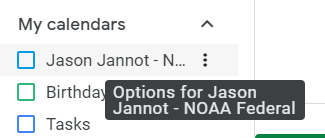
\includegraphics{_img/_gcalendar/pic1.png}

\begin{enumerate}
\def\labelenumi{\arabic{enumi}.}
\setcounter{enumi}{1}
\tightlist
\item
  Click settings and sharing
\end{enumerate}

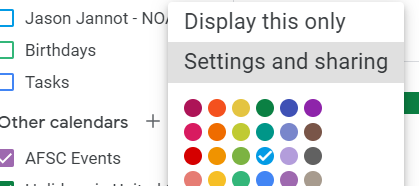
\includegraphics{_img/_gcalendar/pic2.png}

\begin{enumerate}
\def\labelenumi{\arabic{enumi}.}
\setcounter{enumi}{2}
\tightlist
\item
  Make sure to check ``Make available for National Oceanic and
  Atmospheric Administration'' and select ``See all event details'' in
  the drop down.
\end{enumerate}

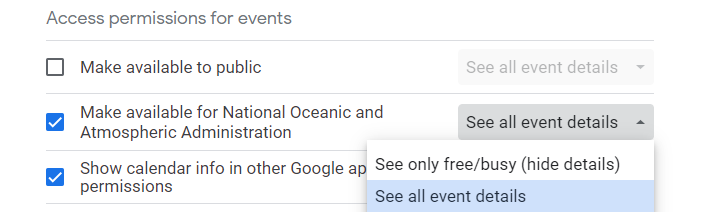
\includegraphics{_img/_gcalendar/pic3.png}

That should do it.

\hypertarget{sec-acronyms}{%
\chapter{Acronyms}\label{sec-acronyms}}

The US Government is absolutely slaphappy about acronyms.

\begin{longtable}[]{@{}
  >{\raggedright\arraybackslash}p{(\columnwidth - 2\tabcolsep) * \real{0.3889}}
  >{\raggedright\arraybackslash}p{(\columnwidth - 2\tabcolsep) * \real{0.6111}}@{}}
\toprule\noalign{}
\begin{minipage}[b]{\linewidth}\raggedright
\textbf{Acronym}
\end{minipage} & \begin{minipage}[b]{\linewidth}\raggedright
\textbf{Definition}
\end{minipage} \\
\midrule\noalign{}
\endhead
\bottomrule\noalign{}
\endlastfoot
AFSC & Alaska Fisheries Science Center \\
AKRO & Alaska Regional Office \\
AMMOP & Alaska Marine Mammal Observer Program \\
A-Team & FMA Analytical Services Program \\
BSAI & Bering Sea Aleutian Islands \\
CAC & Common Access Card, a.k.a., your ``ID badge'' \\
DD & Division Director \\
FMA & Fisheries Monitoring and Analysis Division \\
FMAC & Fishery Monitoring Advisory Committee \\
GOA & Gulf of Alaska \\
M-Team & FMA Management Team = DD, Deputy Director, Debriefing PM,
Training PM, Analytical Services PM \\
NPFMC & North Pacific Fishery Management Council \\
NPOP & North Pacific Observer Program \\
OOO & Out Of Office \\
PCFMAC & Partial Coverage Fishery Monitoring Committee \\
PM & Program Manger \\
PSMFC & Pacific States Marine Fisheries Commission (coloquially,
PacStates) \\
WRC & Western Regional Center, a.k.a., the Sand Point Seattle Campus \\
\end{longtable}

\hypertarget{refs}{}
\begin{CSLReferences}{1}{0}
\leavevmode\vadjust pre{\hypertarget{ref-wilson2017}{}}%
Wilson, Greg, Jennifer Bryan, Karen Cranston, Justin Kitzes, Lex
Nederbragt, and Tracy K. Teal. 2017. {``Good Enough Practices in
Scientific Computing.''} Edited by Francis Ouellette. \emph{PLOS
Computational Biology} 13 (6): e1005510.
\url{https://doi.org/10.1371/journal.pcbi.1005510}.

\end{CSLReferences}



\end{document}
